\documentclass[11pt,a4paper]{article}
\usepackage{polski}
\usepackage[utf8]{inputenc}
\usepackage{graphicx}
\usepackage [colorlinks=true,urlcolor=blue,linkcolor=red,
citecolor=green] {hyperref}
\usepackage[left=2cm,right=2cm,top=1.5cm,bottom=2cm,includeheadfoot,a4paper]{geometry}
\geometry{a4paper}
% by użyć polskich znaków w systemach Linux
% używamy kodowania "latin2" lub "utf8", dla Windows
\title{\Huge{Sounds Good}}
\author{Agnieszka Rudek, Maciej Zienkiewicz, Michał Ulewski}
\date{\today}
\begin{document}
\maketitle
\begin{center}
Prowadzący mgr. inż. Krzysztof Rewak
\end{center}
\begin{figure} [h]
\centering

\includegraphics [scale=0.8]{logo.jpg}
\end{figure}
\newpage
\tableofcontents
\newpage
% pierwsza sekcja
\section{Opis funkcjonalny systemu}\label{sec:tekst}
Aplikacja internetowa \textbf{Sounds Good} została stworzona w celach rozrywkowych na zasadzie quizu. Gra oparta została na losowym utworze z API Spotify.
\section{Zagadnienia zawarte w projekcie}
\subsection{\textbf{HTML5}}
\begin{figure} [h]
\centering
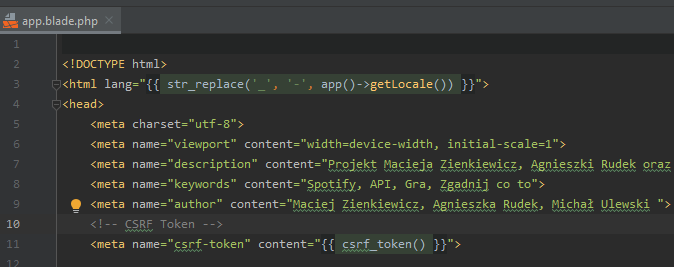
\includegraphics [scale=0.8]{1.1.png}
\end{figure}
\subsection{\textbf{CSS3}}
\begin{figure} [h]
\centering
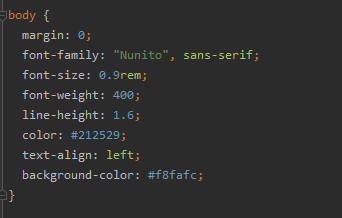
\includegraphics {1.2.png}
\end{figure}
\newpage
\subsection{\textbf{Formularze}}
\begin{figure} [h]
\centering
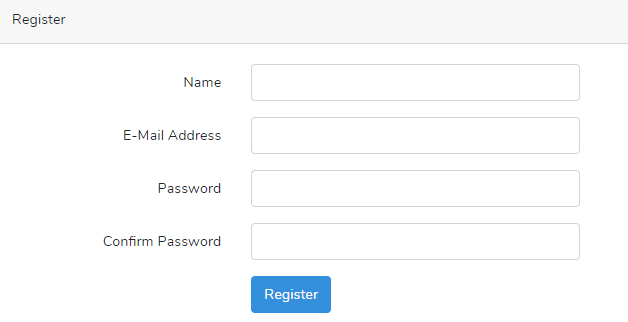
\includegraphics {1.3.png}
\end{figure}
\subsection{\textbf{Baza danych}}
\begin{figure} [h]
\centering
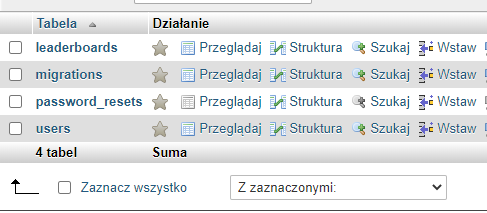
\includegraphics {1.4.png}
\end{figure}
\newpage
\subsection{\textbf{Router}}
\begin{figure} [h]
\centering
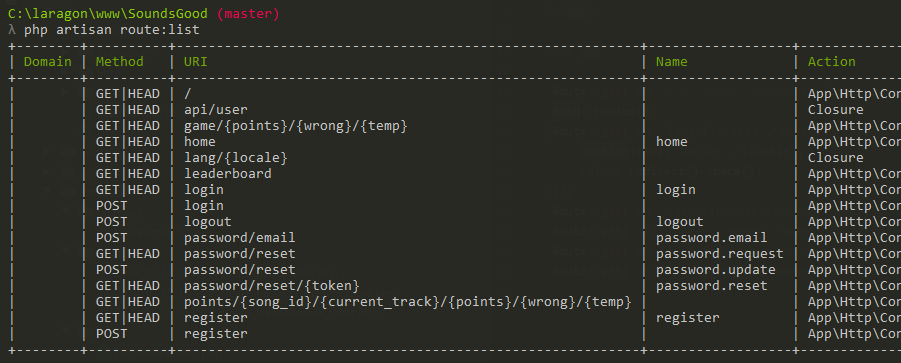
\includegraphics [keepaspectratio, scale=0.7] {1.5.png}
\end{figure}
\begin{figure} [h]
\centering
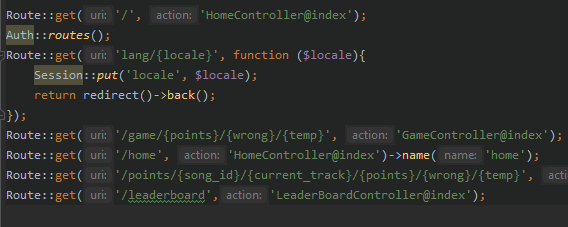
\includegraphics [scale=1] {1.5.1.png}
\end{figure}
\newpage
\subsection{\textbf{Uwierzytelnianie}}
\begin{figure} [h]
\centering
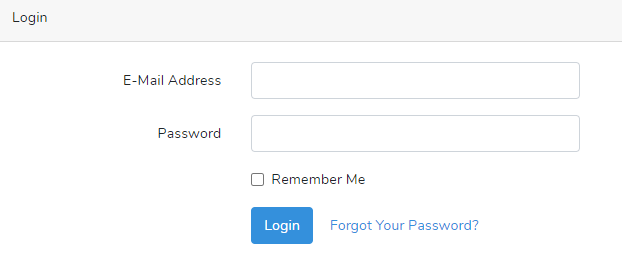
\includegraphics [keepaspectratio] {1.6.png}
\end{figure}
\newpage
\subsection{\textbf{MVC}}
\begin{figure} [h]
\centering
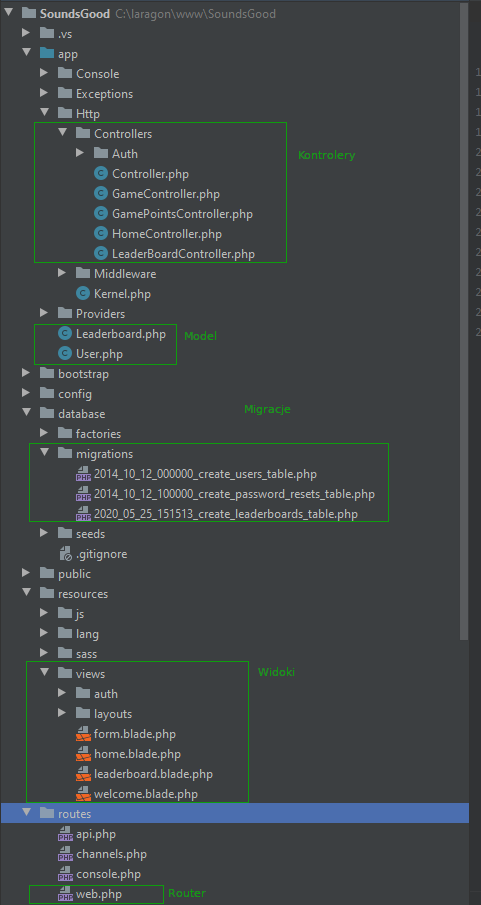
\includegraphics [keepaspectratio, scale=0.75] {1.7.png}
\end{figure}
\newpage
\subsection{\textbf{ORM}}
Wykorzystanie Eloquenta
\begin{figure} [h]
\centering
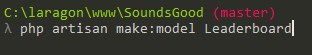
\includegraphics [keepaspectratio] {1.8.1.png}
\end{figure}
\begin{figure} [h]
\centering
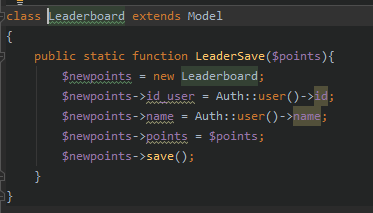
\includegraphics [keepaspectratio] {1.8.png}
\end{figure}
\subsection{\textbf{Konsumowanie API}}
\begin{figure} [h]
\centering
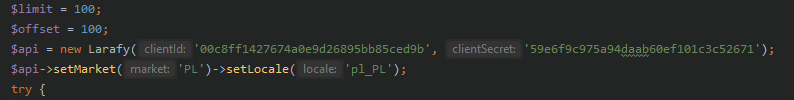
\includegraphics [keepaspectratio, scale=0.8] {1.9.png}
\end{figure}
\newpage
\subsection{\textbf{Mail}}
\begin{figure} [h]
\centering
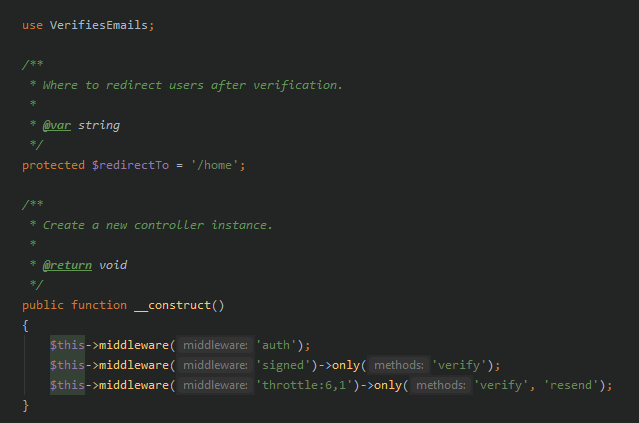
\includegraphics [keepaspectratio] {1.10.png}
\end{figure}
\newpage
\subsection{\textbf{Lokalizacja}}
\begin{figure} [h]
\centering
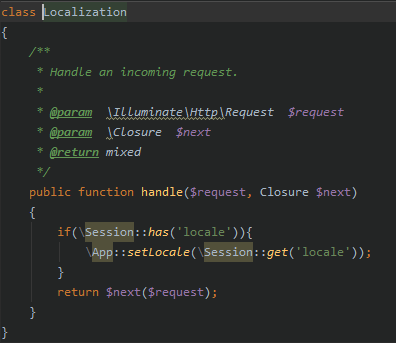
\includegraphics [keepaspectratio] {1.11.png}
\end{figure}
\newpage
\subsection{\textbf{RWD}}
\begin{figure} [h]
\centering
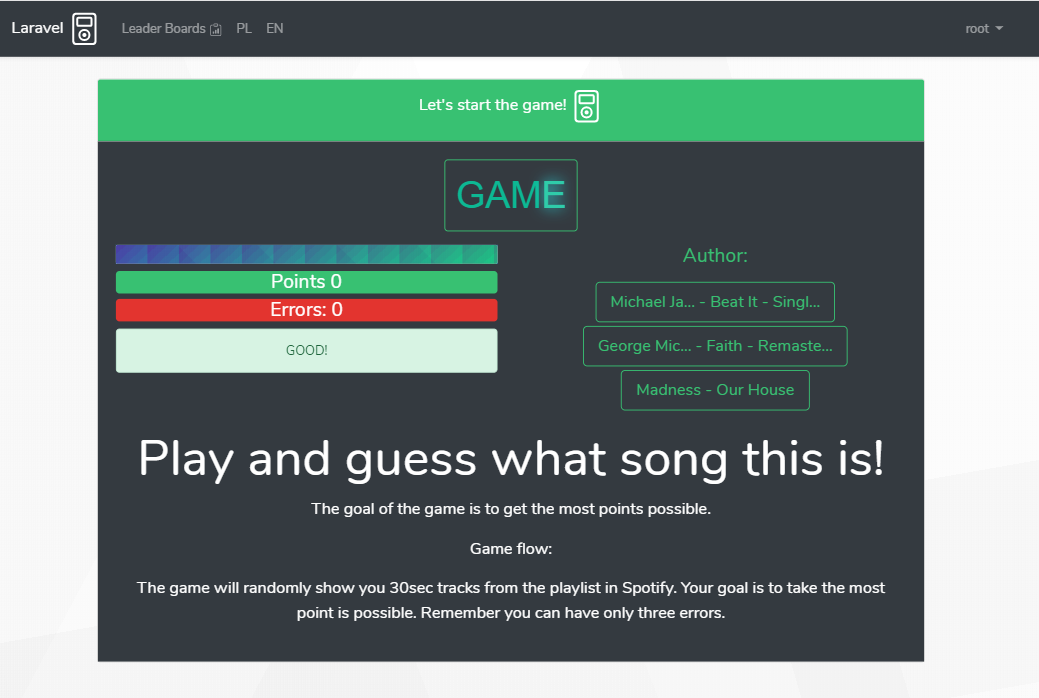
\includegraphics [keepaspectratio, scale=0.6] {1.12.png}
\end{figure}
\begin{figure} [h]
\centering
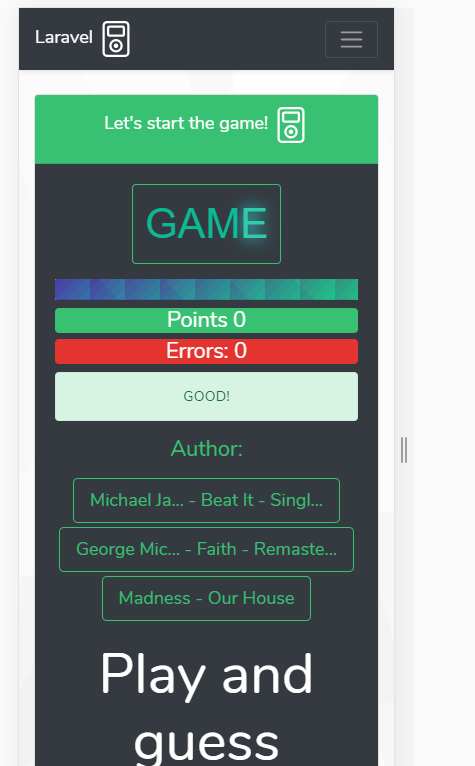
\includegraphics [keepaspectratio, scale=0.9] {1.12.1.png}
\end{figure}
\clearpage
\subsection{\textbf{System zarządzania zależnościami}}
Wykorzystanie Composera do utworzenia projektu
\newline
composer global require laravel/installer
\newline
composer create-project --prefer-dist laravel/laravel blog
\subsection{\textbf{Automatyzacja}}
Wykorzystanie Sass
\begin{figure} [h]
\centering
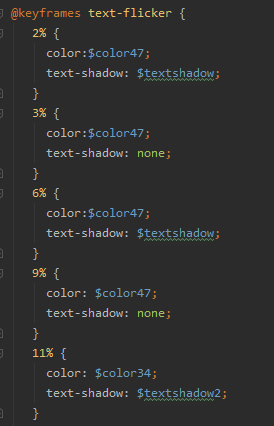
\includegraphics [keepaspectratio, scale=0.9] {1.13.png}
\end{figure}
\subsection{\textbf{SEO}}
\begin{figure} [h]
\centering
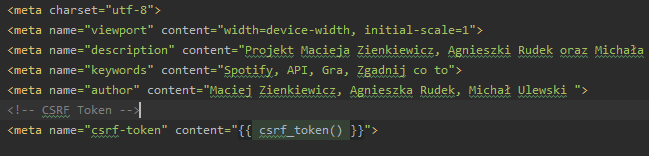
\includegraphics [keepaspectratio, scale=0.9] {1.14.png}
\end{figure}
\newpage
\section{Streszczenie opisu technologicznego}
\begin{itemize}
\item IDE: PHP Storm
\item Menadżer zależności dla PHP - Composer
\item Baza danych MySql i serwer Apache - Laragon
\item Framework back-end PHP - Laravel
\item Framework front-end PHP - Bootstrap
\item Terminal Bash - CMDER
\end{itemize}
\section{Instrukacja lokalnego uruchomienia systemu}
Należy pobrać i zainstalować pakiet \textbf {Laragon}.
\newline
Utworzyć bazę danych w \textbf {phpMyAdmin} o nazwie\textbf {laravel}
\newline
Za pomocą terminala pobrać repozytorum z projektem za pomocą komendy
\newline
\textbf{git clone https://www.github.com/pxmaciej/SoundsGood SoundsGood}
\newline
W terminalu wpisać \textbf  {cp .env example .env}
\newline
W pliku \textbf{.env} uzupełnić dane logowania do bazy danych
\newline
Wpisać komendę generującą nowy klucz: \textbf {php artisan key:generate}
\newline
Wpisac komende migrujaca dane do bazy danych: \textbf {php artisan migrate}
\newline
Wpisac komende tworzaca domyslne obiekty w bazie danych: \textbf {php artisan db:seed}
\newline
Wpisac komende tworzaca domyslne obiekty w bazie danych: \textbf {php artisan serve}
\newline
W przegladarce wejsc na adres \href {http://127.0.0.1:8000} {http://127.0.0.1:8000}
\section{Wnioski projektowe}
PhpStorm jest dobrym narzędziem, które pozwala nam na zachowanie przejrzystości podczas pracy. Posiada bardzo dużo przydatnych funkcji.
Laravel oraz Bootstrap w bardzo dużym stopniu upraszczają pracę ze względu na gotową zawartość, natomiast to czego nam brakuje można bardzo
łatwo doinstalować za pomocą Composera.
\end{document}